\begin{question}[section=11,name={Beverage-Antenne},difficulty=,quantity=,type=thr,tags={20130625}]
	Beschreiben und skizzieren Sie den Aufbau und die Eigenschaften einer Beverage-Antenne. Warum wird diese Antenne nur für Sender kleiner Leistung verwendet?
	
	%\\ \textbf{Hinweis:}\\
	
\end{question}
\begin{solution}
	Die Beverage-Antenne (Langdrahtantenne) hat kein festes Verhältnis von Abmessung zu Wellenlänge. Die Länge beträgt üblicherweise $5$ bis $10\lambda$. Durch einen Abschlusswiderstand erhält die Welle eine ausgeprägte Richtwirkung. Die Antenne wird nur für Sender kleiner Leistungen eingesetzt, weil durch den Abschlusswiderstand der Wirkungsgrad niedrig ist.
	\begin{figure}[H]
		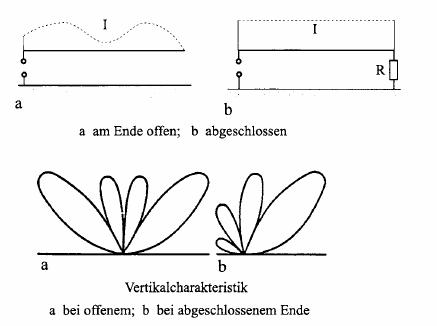
\includegraphics[width=14cm]{./opn/exm/thr/chp/11/1/bild.jpeg}
	\end{figure}
\end{solution}